% Copyright 2004 by Till Tantau <tantau@users.sourceforge.net>.
%
% In principle, this file can be redistributed and/or modified under
% the terms of the GNU Public License, version 2.
%
% However, this file is supposed to be a template to be modified
% for your own needs. For this reason, if you use this file as a
% template and not specifically distribute it as part of a another
% package/program, I grant the extra permission to freely copy and
% modify this file as you see fit and even to delete this copyright
% notice. 

\documentclass{beamer}

\usepackage{docmute}
\usepackage{pgfgantt}
\usepackage{graphicx}

\usepackage[utf8]{inputenc}
\usepackage[hungarian]{babel}

% There are many different themes available for Beamer. A comprehensive
% list with examples is given here:
% http://deic.uab.es/~iblanes/beamer_gallery/index_by_theme.html
% You can uncomment the themes below if you would like to use a different
% one:

\usetheme{Hannover}


\title{Kell ide egy cím}

% A subtitle is optional and this may be deleted
\subtitle{A statisztikus gépi fordítás hatékonyságának jelentés egyértelműsítéssel történő javítása}

\author{E.~Bordi, T.~Both, Sz.~Pável, Cs.~Sándor, A.~Szász}
% - Give the names in the same order as the appear in the paper.
% - Use the \inst{?} command only if the authors have different
%   affiliation.

\institute[Babe\c{s}-Bolyai Tudományegyetem] % (optional, but mostly needed)
{Babe\c{s}-Bolyai Tudományegyetem, Matematika és Informatika Kar, Kolozsvár}
% - Use the \inst command only if there are several affiliations.
% - Keep it simple, no one is interested in your street address.

\date{2016 április 15.}
% - Either use conference name or its abbreviation.
% - Not really informative to the audience, more for people (including
%   yourself) who are reading the slides online 

% If you have a file called "university-logo-filename.xxx", where xxx
% is a graphic format that can be processed by latex or pdflatex,
% resp., then you can add a logo as follows:

% \pgfdeclareimage[height=0.5cm]{university-logo}{university-logo-filename}
% \logo{\pgfuseimage{university-logo}}

% Delete this, if you do not want the table of contents to pop up at
% the beginning of each subsection:
\AtBeginSubsection[]
{
  \begin{frame}<beamer>{Tartalom}
    \tableofcontents[currentsection,currentsubsection]
  \end{frame}
}

% Let's get started
\begin{document}


% Sections are stored in separate .tex files
\begin{frame}
  \titlepage
\end{frame}
\begin{frame}{Tartalom}
  \tableofcontents
  % You might wish to add the option [pausesections]
\end{frame}
\section{Motiváció}
\begin{frame}{Motiváció}
\begin{itemize}
  \item {Gépi fordítás: elsősorban szövegek megértésének elősegítésére, információszerzésre használják, jelenleg nem alkalmas emberi fordítással azonos minőségű fordítás létrehozására.}
  \item {Főbb nehézségek:}
  \begin{itemize}
  \item {Többértelmű szavak fordítása}
  \item {Kifejezések fordítása}
  \item {Szintaktikai nehézségek}
  \end{itemize}
  
\end{itemize}

\end{frame}
\section{Kutatási terv}
\subsection{Csapat tagjainak hozzájárulása}

\begin{frame}{Csapat tagjainak hozzájárulása}

\begin{table}
\begin{tabular}{l | c }
Feladatkör & Csapattag\\
\hline \hline
Megvalósítandó anyagok & {\color{blue}Bordi Eszter}\\
Munkabeosztás & \\
Gantt diagram & \\
Motiváció & {\color{blue}Both Tibor}\\ 
Megtenni szándékozott lépések & {\color{blue}Pável Szabolcs}\\
Létező megoldások & {\color{blue}Sándor Csanád}\\
Csapat tagjainak hozzájárulása & {\color{blue}Szász Adorján}
\end{tabular}
\end{table}

\end{frame}
\subsection{Megtenni szándékozott lépések}

\begin{frame}{Megtenni szándékozott lépések}
	
	\begin{itemize}
		
		\item Wikipedia alapú WSD rendszer felépítése
		\begin{enumerate}
			\item Egyik legnagyobb létező adathalmaz
			\item Több nyelven elérhető
			\item A cikkek címei concept-ként való felhasználása
		\end{enumerate}
		
		\item WSD rendszer integrálása a létező SMT rendszerekbe
		\begin{enumerate}
			\item Statisztikai modellek nem veszik figyelembe a  többértelmű szavakat
			\item A fordítás pontossága nagyban növelhető lenne ezen problémák megoldásával
		\end{enumerate}
		
	\end{itemize}

\end{frame}

\newcounter{enumcounter}
\newcommand{\savecounter}{\setcounter{enumcounter}{\theenumi}}
\newcommand{\restorecounter}{\setcounter{enumi}{\theenumcounter}}

\begin{frame}{Megtenni szándékozott lépések}
\framesubtitle{Wikipedia alapú WSD rendszer}

		\begin{enumerate}
			\item Invertált index felépítése minden nyelv számára	
			\begin{itemize}
				\item Minden szóhoz hozzárendelünk concept-eket és a hozzájuk tartozó súlyt
				\item A concept-ek az angol Wikipedia címek
				\item Súlyozáshoz használhatjuk például a tf-idf súlyozást
			\end{itemize}			
			
		\begin{figure}[t]
			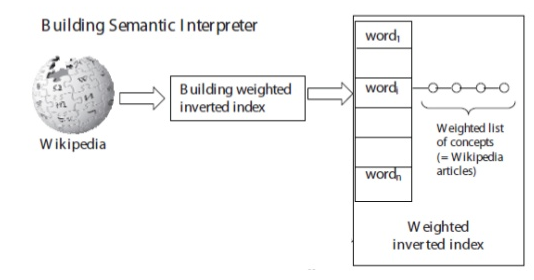
\includegraphics[scale=0.4]{images/invindex}
 		\end{figure}			
			
			\savecounter	
		\end{enumerate}

\end{frame}

\begin{frame}{Megtenni szándékozott lépések}
\framesubtitle{Wikipedia alapú WSD rendszer}

	\begin{enumerate}
		\restorecounter
		
		\item Súlyozott concept vektor hozzárendelése a fordítandó és SMT által fordított szöveghez
		\begin{itemize}
			\item Szöveg szavak vektoraként való ábrázolása 
			\item Concept-ek megfelelő súllyal történő hozzárendelése minden szóhoz
			\item Ősszesített súlyozott concept lista felépítése a szöveghez
		\end{itemize}
		
		\begin{figure}[t]
			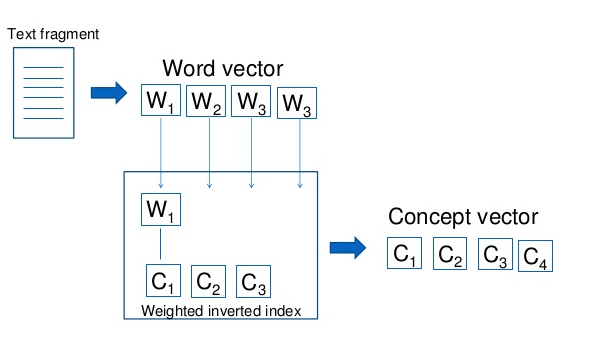
\includegraphics[scale=0.4]{images/textfragment}
 		\end{figure}			
 		
	\savecounter
 	
	\end{enumerate}
	
\end{frame}

\begin{frame}{Megtenni szándékozott lépések}
\framesubtitle{Wikipedia alapú WSD rendszer}

	\begin{enumerate}
		\restorecounter	
	
		\item A szemantikai hasonlóság meghatározza a fordítandó és célszöveg között
		\begin{itemize}
			\item A fordítandó- és célszöveghez felépítjük a concept vektorokat
			\item A hasonlóság vizsgálatát a vektorok összehasonlítása jelenti
			\item A hasonlósági metrika lehet például a gyakran használt cos-távolság
		\end{itemize}
	
		\begin{figure}[t]
			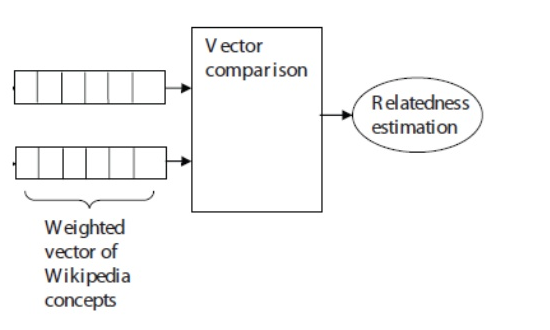
\includegraphics[scale=0.4]{images/similarity}
 		\end{figure}	
	
		\savecounter
	\end{enumerate}

\end{frame}

\begin{frame}{Megtenni szándékozott lépések}
\framesubtitle{WSD súlyok integrálása}	
	
	\begin{enumerate}
		\restorecounter
						
		\item Legjobb N találat újrarangsorolása
		\begin{itemize}
			\item SMT rendszer alapján meghatározni a legjobb N fordítást
			\item WSD rendszer alapján súly hozzárendelése a találatokhoz
			\item A találatok újrarangsorolása az SMT és WSD együttes eredményei alapján
		\end{itemize}
	\end{enumerate}
	
\end{frame}
\begin{frame}{Outline}
  \tableofcontents
  % You might wish to add the option [pausesections]
\end{frame}
\setbeamercovered{transparent}

\definecolor{barblue}{RGB}{153,204,254}
\definecolor{groupblue}{RGB}{51,102,254}
\definecolor{linkred}{RGB}{165,0,33}
\renewcommand\sfdefault{phv}
\renewcommand\mddefault{mc}
\renewcommand\bfdefault{bc}
\setganttlinklabel{s-s}{START-TO-START}
\setganttlinklabel{f-s}{FINISH-TO-START}
\setganttlinklabel{f-f}{FINISH-TO-FINISH}
\sffamily

\subsection{Munkabeosztás és ütemterv}

% % % % % % % % % % % % % % % % % % % % % % % % %
% MUNKAEGYSÉGEK
% % % % % % % % % % % % % % % % % % % % % % % % %
\begin{frame}{Munkabeosztás és ütemterv}
Munkaegységek:
\begin{itemize}
  \item {A kutatás beindítása, adatgyűjtés}
  \item {Az adathalmaz összeállítása}
  \item {Algoritmus kidolgozása}
  \item {Az új és régi módszerek összevetése}
  \item {Az algoritmus optimalizálása, prototípus-fejlesztés}
  \end{itemize}
\end{frame}


% % % % % % % % % % % % % % % % % % % % % % % % %
%RÉSZFELADATOK 1
% % % % % % % % % % % % % % % % % % % % % % % % %
\begin{frame}{Munkabeosztás és ütemterv}
Munkaegységek és részfeladatai:
\begin{itemize}
  \item<1-> {
    A kutatás beindítása, adatgyűjtés
    \begin{enumerate}
	    \item Kutatási módszertani lehetőségek felvázolása
	    \item Kutatási terv kidolgozása
	    \item Meglévő módszerek feltérképezése
	    \item Prototípus első koncepciójának kidolgozása
    \end{enumerate}
  }
  \item<2-> {   
    Az adathalmaz összeállítása
    \begin{enumerate}
        \item Adatok gyűjtése
        \item Standard formátumra való alakítás
        \item Adathalmaz validálása
    \end{enumerate}
  }
  \item<3-> {
    Algoritmus kidolgozása
    \begin{enumerate}
        \item Algoritmus leírása
        \item Teszt jegyzőkönyvek, a statisztikus gépi fordítás hatékonyságával kapcsolatos hatások vizsgálata
    \end{enumerate}
  }
  \end{itemize}
\end{frame}

% % % % % % % % % % % % % % % % % % % % % % % % %
%RÉSZFELADATOK 2
% % % % % % % % % % % % % % % % % % % % % % % % %
\begin{frame}{Munkabeosztás és ütemterv}
Munkaegységek és részfeladatai:
\begin{itemize}
  \item<1-> {
    Az új és régi módszerek összevetése
    \begin{enumerate}
        \item Tesztfuttatások különböző algoritmusokkal és adatokkal, a statisztikus gépi fordítás hatékonyságával kapcsolatos hatások vizsgálata
        \item Az eltérés statisztikus validációja
        \item Szintézis
    \end{enumerate}
  }
  \item<2-> {
    Az algoritmus optimalizálása, prototípus-fejlesztés
    \begin{enumerate}
        \item Performanciaoptimalizált algoritmus
        \item A gépi fordító prototípusának tesztelése és tesztjegyzőkönyvek
        \item Nyilvánosságra hozandó eredmények dokumentációja
        \item A projekt lezárása, dokumentáció
    \end{enumerate}
  }
  \end{itemize}
\end{frame}

% % % % % % % % % % % % % % % % % % % % % % % % %
%GANTT
% % % % % % % % % % % % % % % % % % % % % % % % %
\begin{frame}{Munkabeosztás és ütemterv}
	\begin{ganttchart}[
	x unit=0.4cm,
	y unit title=1cm,
	y unit chart=0.5cm,
	    canvas/.append style={fill=none, draw=black!5, line width=.75pt},
	    hgrid style/.style={draw=black!5, line width=.75pt},
	    vgrid={*1{draw=black!5, line width=.75pt}},
	    today=7,
	    today rule/.style={
	      draw=black!64,
	      dash pattern=on 3.5pt off 4.5pt,
	      line width=1.5pt
	    },
	    today label font=\small\bfseries,
	    title/.style={draw=none, fill=none},
	    title label font=\bfseries\footnotesize,
	    title label node/.append style={below=7pt},
	    include title in canvas=false,
	    bar label font=\mdseries\small\color{black!70},
	    bar label node/.append style={left=2cm},
	    bar/.append style={draw=none, fill=black!63},
	    bar incomplete/.append style={fill=barblue},
	    bar progress label font=\mdseries\tiny\color{black!70},
	    group incomplete/.append style={fill=groupblue},
	    group left shift=0,
	    group right shift=0,
	    group height=.5,
	    group peaks tip position=0,
	    group label node/.append style={left=.6cm},
	    group progress label font=\bfseries\tiny,
	    link/.style={-latex, line width=1.5pt, linkred},
	    link label font=\scriptsize\bfseries,
	    link label node/.append style={below left=-2pt and 0pt}
	  ]{1}{13}
	  \gantttitle[
	    title label node/.append style={below left=7pt and -3pt}
	  ]{HÉT:\quad1}{1}
	  \gantttitlelist{2,...,14}{1} \\
	  \ganttgroup[progress=57]{WBS 1 Summary Element 1}{1}{10} \\
	  \ganttbar[
	    progress=75,
	    name=WBS1A
	  ]{\textbf{WBS 1.1} Activity A}{1}{8} \\
	  \ganttbar[
	    progress=67,
	    name=WBS1B
	  ]{\textbf{WBS 1.2} Activity B}{1}{3} \\
	  \ganttbar[
	    progress=50,
	    name=WBS1C
	  ]{\textbf{WBS 1.3} Activity C}{4}{10} \\
	  \ganttbar[
	    progress=0,
	    name=WBS1D
	  ]{\textbf{WBS 1.4} Activity D}{4}{10} \\[grid]
	  \ganttgroup[progress=0]{WBS 2 Summary Element 2}{4}{10} \\
	  \ganttbar[progress=0]{\textbf{WBS 2.1} Activity E}{4}{5} \\
	  \ganttbar[progress=0]{\textbf{WBS 2.2} Activity F}{6}{8} \\
	  \ganttbar[progress=0]{\textbf{WBS 2.3} Activity G}{9}{10}
%	  \ganttlink[link type=s-s]{WBS1A}{WBS1B}
%	  \ganttlink[link type=f-s]{WBS1B}{WBS1C}
%	  \ganttlink[
%	    link type=f-f,
%	    link label node/.append style=left
%	  ]{WBS1C}{WBS1D}
	\end{ganttchart}
\end{frame}


% Section and subsections will appear in the presentation overview
% and table of contents.
%\section{First Main Section}
%
%\subsection{First Subsection}
%
%\begin{frame}{First Slide Title}{Optional Subtitle}
%  \begin{itemize}
%  \item {
%    My first point.
%  }
%  \item {
%    My second point.
%  }
%  \end{itemize}
%\end{frame}
%
%\subsection{Second Subsection}
%
%% You can reveal the parts of a slide one at a time
%% with the \pause command:
%\begin{frame}{Second Slide Title}
%  \begin{itemize}
%  \item {
%    First item.
%    \pause % The slide will pause after showing the first item
%  }
%  \item {   
%    Second item.
%  }
%  % You can also specify when the content should appear
%  % by using <n->:
%  \item<3-> {
%    Third item.
%  }
%  \item<4-> {
%    Fourth item.
%  }
%  % or you can use the \uncover command to reveal general
%  % content (not just \items):
%  \item<5-> {
%    Fifth item. \uncover<6->{Extra text in the fifth item.}
%  }
%  \end{itemize}
%\end{frame}
%
%\section{Second Main Section}
%
%\subsection{Another Subsection}
%
%\begin{frame}{Blocks}
%\begin{block}{Block Title}
%You can also highlight sections of your presentation in a block, with it's own title
%\end{block}
%\begin{theorem}
%There are separate environments for theorems, examples, definitions and proofs.
%\end{theorem}
%\begin{example}
%Here is an example of an example block.
%\end{example}
%\end{frame}
%
%% Placing a * after \section means it will not show in the
%% outline or table of contents.
%\section*{Summary}
%
%\begin{frame}{Summary}
%  \begin{itemize}
%  \item
%    The \alert{first main message} of your talk in one or two lines.
%  \item
%    The \alert{second main message} of your talk in one or two lines.
%  \item
%    Perhaps a \alert{third message}, but not more than that.
%  \end{itemize}
%  
%  \begin{itemize}
%  \item
%    Outlook
%    \begin{itemize}
%    \item
%      Something you haven't solved.
%    \item
%      Something else you haven't solved.
%    \end{itemize}
%  \end{itemize}
%\end{frame}



% All of the following is optional and typically not needed. 
\appendix
\section<presentation>*{\appendixname}
\subsection<presentation>*{For Further Reading}

\begin{frame}[allowframebreaks]
  \frametitle<presentation>{For Further Reading}
    
  \begin{thebibliography}{10}
    
  \beamertemplatebookbibitems
  % Start with overview books.

  \bibitem{Author1990}
    A.~Author.
    \newblock {\em Handbook of Everything}.
    \newblock Some Press, 1990.
 
    
  \beamertemplatearticlebibitems
  % Followed by interesting articles. Keep the list short. 

  \bibitem{Someone2000}
    S.~Someone.
    \newblock On this and that.
    \newblock {\em Journal of This and That}, 2(1):50--100,
    2000.
  \end{thebibliography}
\end{frame}

\end{document}


